% Capítulo 1 (Problema) — Slide 2 — Heterogeneidade da demanda (figura isolada)
\begin{frame}{Heterogeneidade da demanda}
  \centering
  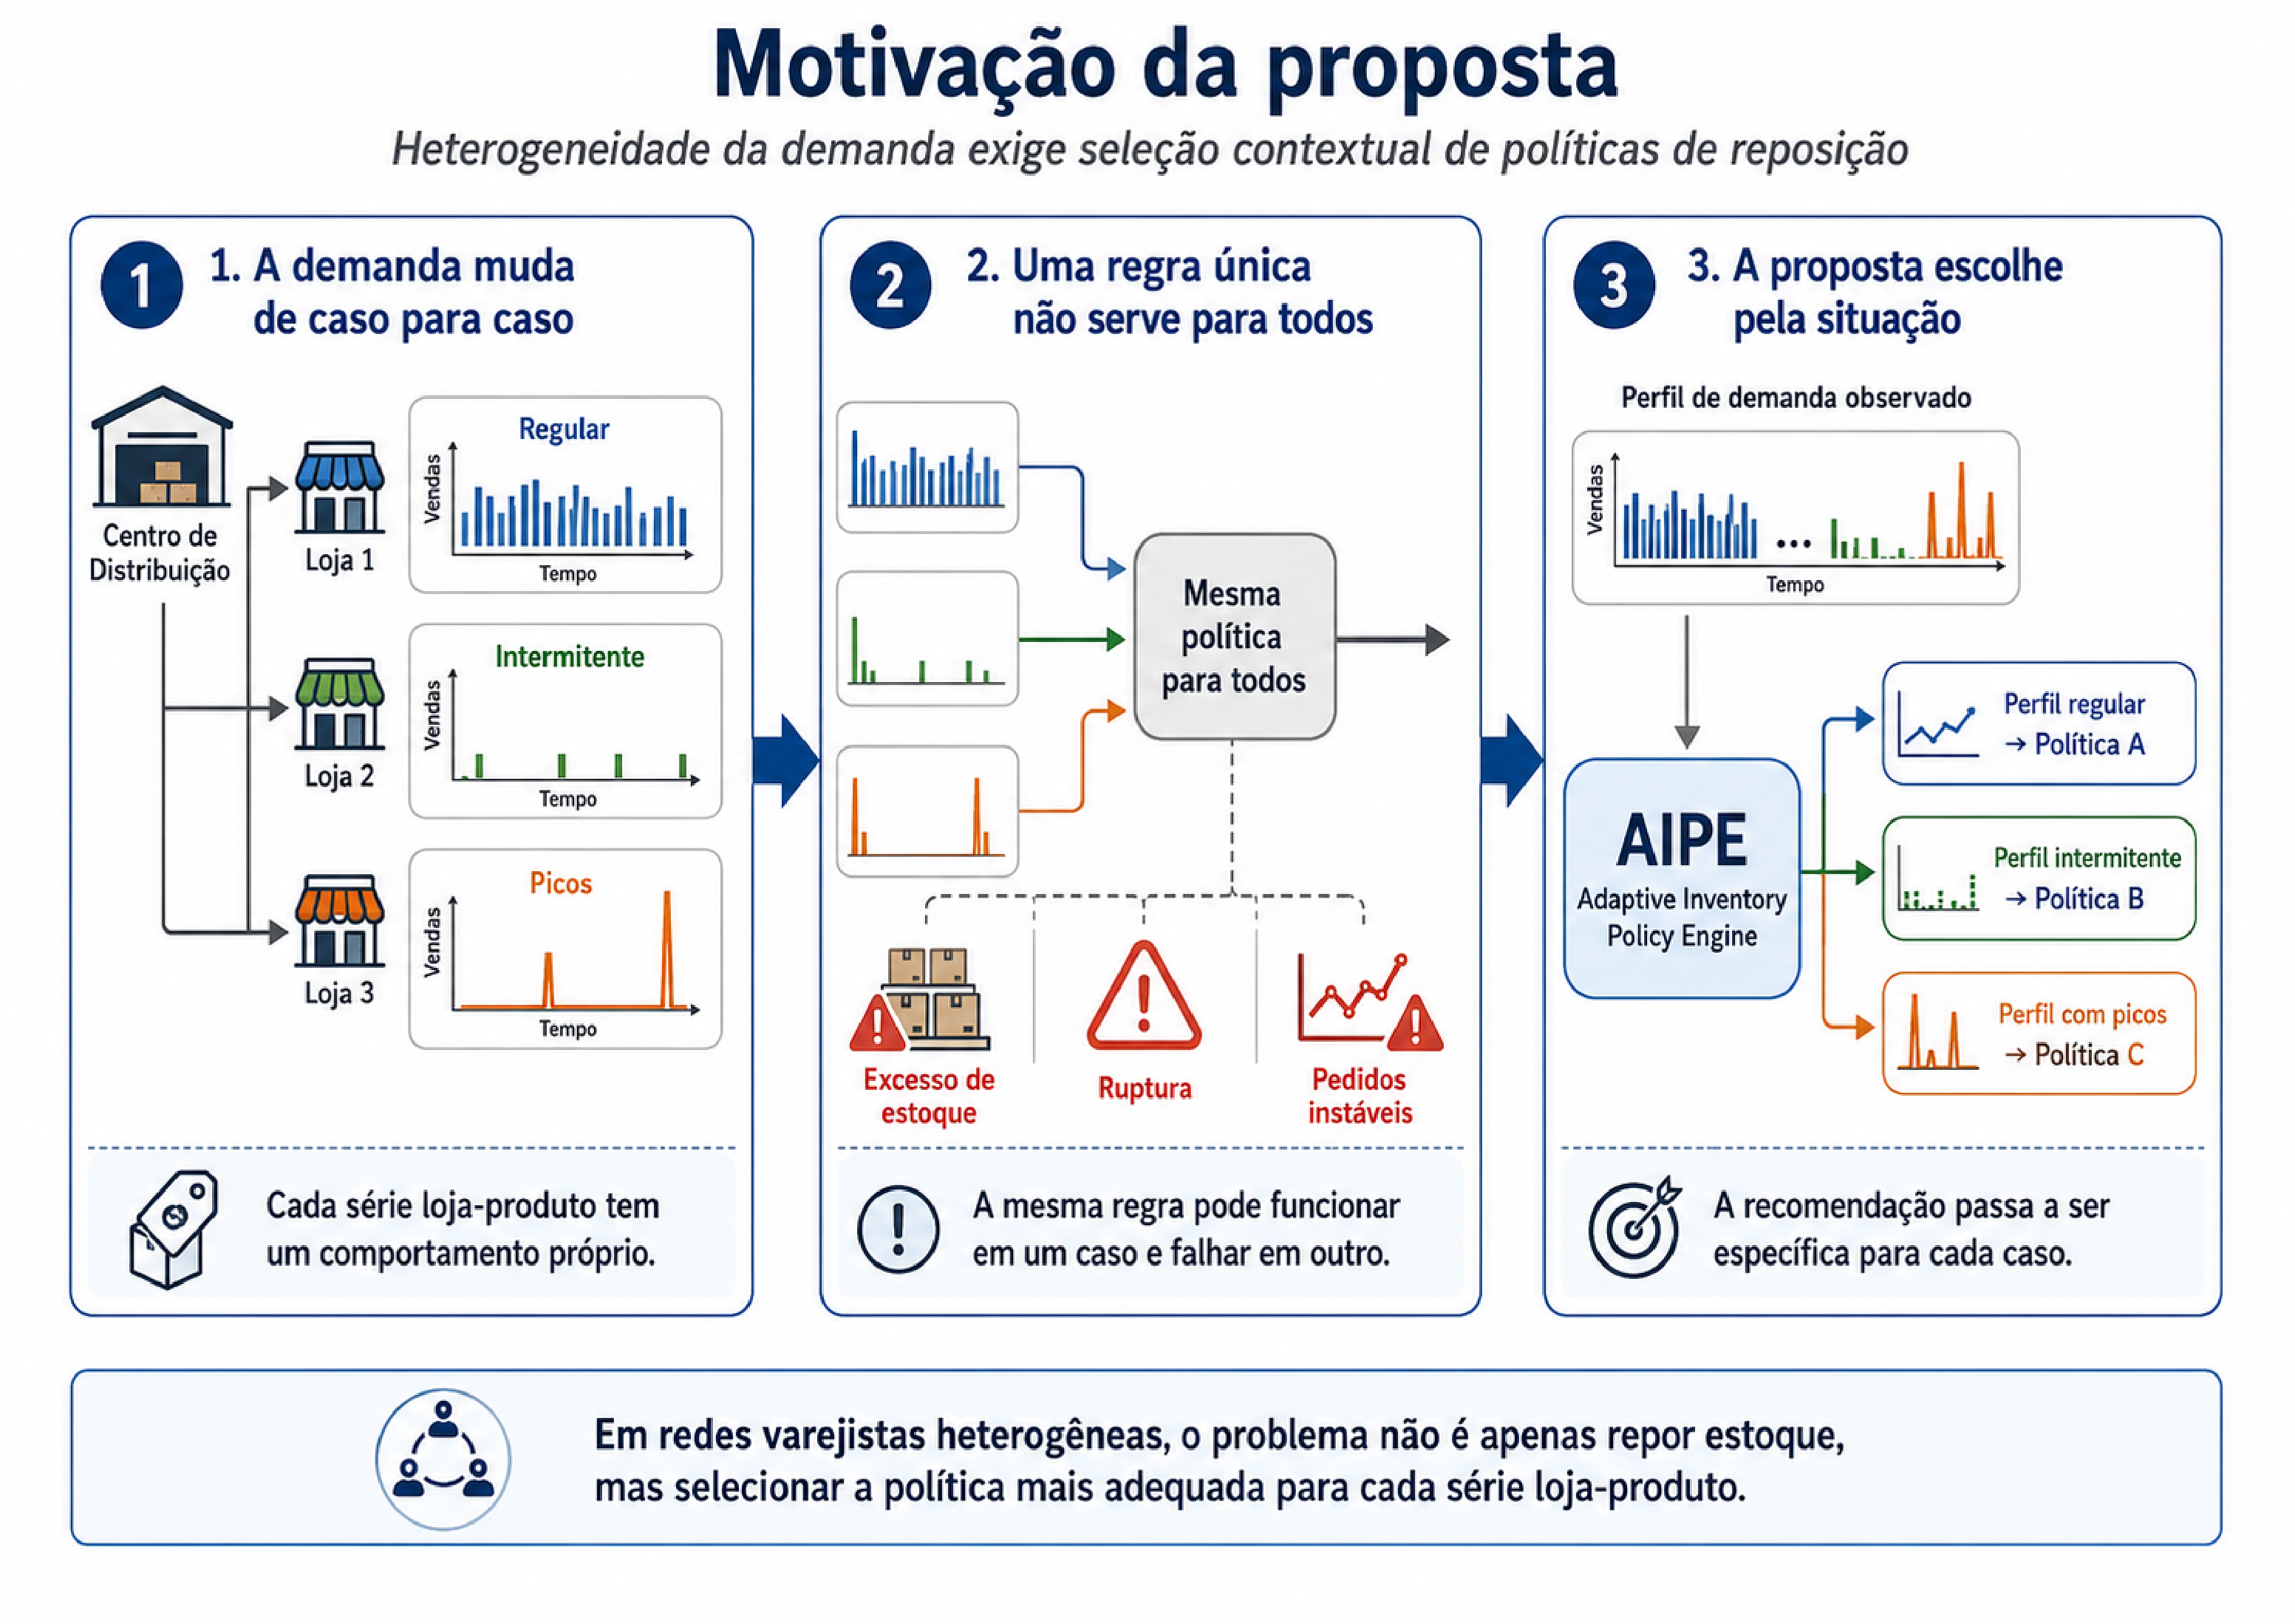
\includegraphics[width=0.99\linewidth,height=6.95cm,keepaspectratio]{figures/figura_1_1_motivacao_aipe.pdf}
  \note{
    Esta figura, do Capítulo 1 da dissertação, ilustra a heterogeneidade que
    motiva o trabalho. Dentro da mesma rede, um produto pode vender de forma
    regular e previsível -- por exemplo, 50 unidades por semana em qualquer
    loja -- enquanto outro apresenta um padrão intermitente, do tipo
    ``0, 0, 0, 50, 0, 0, 30'', com longos períodos de demanda nula
    intercalados por picos esporádicos. Aplicar a mesma regra de reposição a
    esses dois casos tende a ser ineficiente: o que funciona bem para a
    demanda regular pode gerar excesso de estoque ou ruptura na demanda
    intermitente. A proposta investigada nesta dissertação -- selecionar
    políticas de forma contextual -- nasce diretamente dessa observação.
  }
\end{frame}
